\chapter{DISEÑO CONCEPTUAL}\label{cap:diseno-conceptual}
\listasdecapitulo{3}

En este capítulo se establece la base conceptual de un sistema de control adaptativo inteligente para la red
semafórica vial de Lima. Siguiendo la metodología de diseño VDI 2221, se parte del análisis de los actores y
sus necesidades, se deriva una lista de requerimientos verificable, se modela el sistema como una caja negra,
se descompone su estructura funcional, y mediante una matriz morfológica se generan y evalúan conceptos
completos hasta seleccionar la solución óptima. El propósito es responder a la problemática del sistema
semafórico actual, caracterizado por ineficiencia, descoordinación y falta de adaptabilidad al flujo
vehicular.

\textbf{Qué queda fijo y qué se valida.} El diseño conceptual fija las decisiones de arquitectura del sistema
y no se modifican en los capítulos posteriores: (i) una arquitectura complementaria \emph{edge}--nube en la
que el módulo IoT recomienda y el controlador semafórico existente conserva la \textbf{autoridad final} sobre
luces y enclavamientos; (ii) el sensado principal basado en \textbf{una única cámara} con visión por
computadora; (iii) la estimación local de un índice de congestión y un \textbf{control difuso} como estrategia
de adaptación; (iv) la comunicación segura con la nube para supervisión, histórico y coordinación no crítica;
y (v) la validación mediante \textbf{SUMO} frente a una línea base. En cambio, los \emph{valores de
ingeniería} (protecciones y autonomía energética, grado IP y geometría del gabinete, altura y cobertura de la
cámara, parámetros del controlador difuso, métricas de desempeño y costos) se calculan, dimensionan y
\textbf{validan} en los Capítulos~4 a~7. Esta separación evita afirmar resultados antes de obtenerlos y
mantiene el diseño conceptual como marco estable de las etapas siguientes.

\section{Actores clave y necesidades}\label{sec:actores-necesidades}

Los actores clave del sistema se identificaron a partir de entrevistas con expertos y encuestas a usuarios del
sistema actual. Comprenden al cliente principal (la Municipalidad Metropolitana de Lima), los usuarios finales
directos (conductores y peatones), los usuarios indirectos (operativos de tránsito y administradores de la
infraestructura) y los interesados secundarios (autoridades de seguridad vial). La Tabla~\ref{tab:actores}
sintetiza sus necesidades.

\begin{table}[H]
  \centering
  \footnotesize
  \caption{Actores clave del sistema y sus necesidades principales.}
  \label{tab:actores}
  \begin{tabularx}{\linewidth}{@{}>{\raggedright\arraybackslash}p{4.3cm}>{\raggedright\arraybackslash}X@{}}
    \toprule
    \textbf{Actor} & \textbf{Necesidades principales}\\
    \midrule
    Cliente (Municipalidad / Subgerencia de Movilidad Urbana) &
    Coordinación y eficiencia de la red en tiempo real mediante ajuste dinámico de ciclos según el flujo;
    monitoreo en tiempo real interpretable, con alertas sobre incidencias y desviaciones del tráfico.\\
    Usuarios finales (conductores y peatones) &
    Reducir tiempos de espera y mejorar la fluidez, en especial en intersecciones con semáforos mal
    coordinados; mejorar la seguridad vial reduciendo accidentes y conductas temerarias asociadas a la
    frustración.\\
    Usuarios indirectos (operativos y administradores de infraestructura) &
    Comunicación centralizada para supervisar y sincronizar intersecciones desde un punto único; medidas de
    ciberseguridad que protejan la integridad y confidencialidad de los datos.\\
    Usuarios directos y operativos (autoridades de tránsito) &
    Interfaz gráfica intuitiva con alertas automáticas y datos en tiempo real que permitan un ajuste ágil y
    decisiones rápidas ante situaciones imprevistas.\\
    \bottomrule
  \end{tabularx}
  \fuente{Elaboración propia.}
\end{table}

Las respuestas de la encuesta a usuarios finales respaldan estas necesidades: el 60\,\% consideró muy
importante la reducción de tiempos de espera, el 40\,\% destacó la sincronización entre semáforos como aspecto
clave y el 50\,\% asoció las conductas peligrosas a la frustración causada por el sistema semafórico actual.

\section{Lista de requerimientos}\label{sec:requerimientos}

A partir de las necesidades anteriores se derivan los requerimientos del sistema, clasificados como exigencias
(obligatorias) o deseos (mejoras adicionales), y se traducen en una \textbf{especificación verificable
codificada} donde cada requerimiento recibe un código, un valor objetivo, su justificación, el método de
verificación previsto y una prioridad M (mandatoria), A (alta) o D (deseable), conforme a la estructura VDI
2221. Esta especificación consolidada gobierna el resto de la tesis y se presenta íntegra, junto con el
resumen de exigencias y deseos por dominio de diseño, en el Anexo~A (Tablas~\ref{tab:exigencias}
y~\ref{tab:req-verificables}).

\section{Estructura de funciones}\label{sec:estructura-funciones}

\subsection{Frontera del sistema y modelo de caja negra}\label{sec:caja-negra}

La frontera del sistema se fija alrededor del módulo IoT complementario. El controlador semafórico existente y
la plataforma en la nube son sistemas externos con los que se intercambian señales; las lámparas y sus
enclavamientos permanecen bajo responsabilidad del controlador vial. La Figura~\ref{fig:caja-negra} representa
el sistema como una caja negra, en la que las líneas punteadas representan señales, las líneas delgadas la
energía y las líneas gruesas la materia.

\begin{figure}[H]
  \centering
  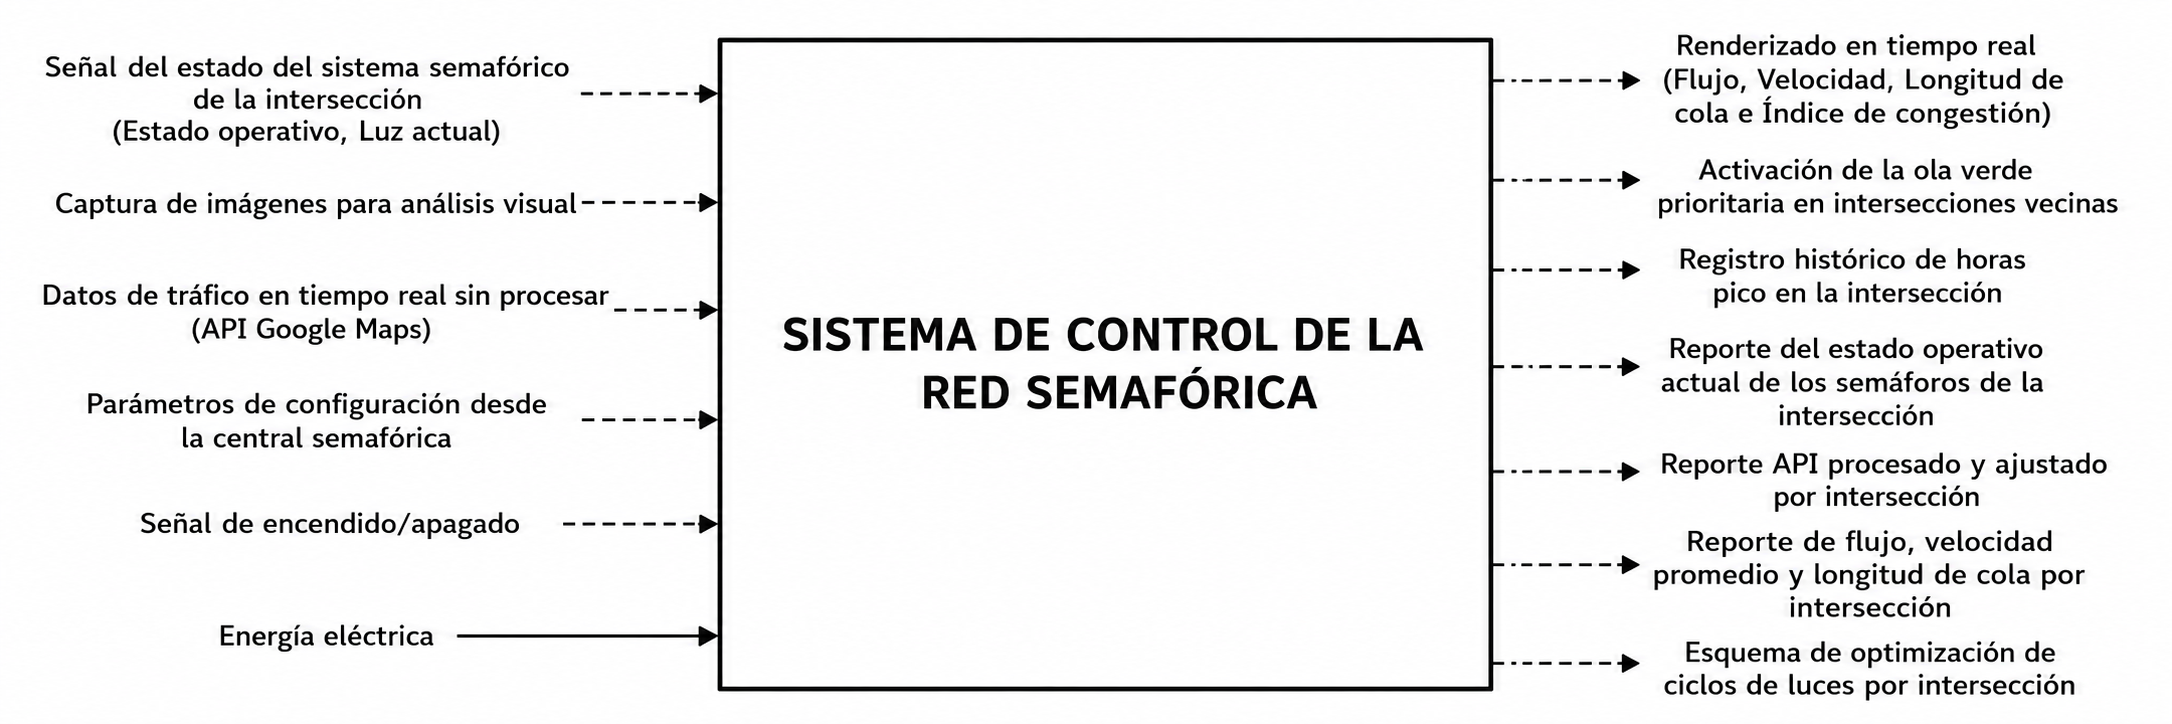
\includegraphics[width=0.9\linewidth,keepaspectratio]{media/image91.png}
  \caption{Caja negra del sistema y frontera de responsabilidad del módulo IoT complementario.}
  \label{fig:caja-negra}
  \fuente{Elaboración propia.}
\end{figure}

La Tabla~\ref{tab:entradas-salidas} consolida las entradas y salidas del sistema con su uso dentro de la
arquitectura, evitando duplicar en prosa el detalle de cada señal.

\begin{table}[H]
  \centering
  \footnotesize
  \caption{Entradas y salidas del módulo IoT y su uso dentro de la arquitectura.}
  \label{tab:entradas-salidas}
  \begin{tabularx}{\linewidth}{@{}>{\raggedright\arraybackslash}p{1.7cm}>{\raggedright\arraybackslash}p{5.0cm}>{\raggedright\arraybackslash}X@{}}
    \toprule
    \textbf{Tipo} & \textbf{Variable o flujo} & \textbf{Uso dentro de la arquitectura}\\
    \midrule
    Entrada & Imagen o video de la cámara & Estimar conteo, velocidad, ocupación, cola y calidad del sensado.\\
    Entrada & Sensores auxiliares y diagnóstico eléctrico/ambiental & Detectar condiciones internas anómalas y apoyar el mantenimiento.\\
    Entrada & Estado del controlador semafórico & Sincronizar recomendaciones con la fase vigente sin sustituir sus enclavamientos.\\
    Entrada & Parámetros autorizados e históricos & Configurar límites, pesos y referencias dentro de rangos validados.\\
    Entrada & Restricciones de seguridad y estado de conectividad & Seleccionar modo normal, degradado o retorno al plan base.\\
    Entrada & Energía eléctrica & Alimentar de forma estable y continua a todos los componentes.\\
    Salida & Índice de congestión y variables de tráfico & Entradas verificables para el control difuso y la supervisión.\\
    Salida & Parámetros sugeridos de fase & Recomendación acotada que debe ser validada por la autoridad final.\\
    Salida & Telemetría, alertas, reportes y estado del módulo & Operación, mantenimiento, auditoría y análisis histórico.\\
    Salida & Registro local e histórico remoto & Evidencia para trazabilidad, diagnóstico y calibración.\\
    \bottomrule
  \end{tabularx}
  \fuente{Elaboración propia.}
\end{table}

\subsection{Descomposición funcional por dominios}\label{sec:dominios-funcionales}

La estructura funcional se organiza en dominios complementarios: \textbf{sensado}, que capta la escena vial;
\textbf{procesamiento local}, que preprocesa y estima variables; \textbf{control}, que calcula el ajuste
difuso y aplica restricciones; \textbf{comunicación}, que intercambia mensajes; \textbf{nube}, que supervisa y
conserva históricos; \textbf{ciberseguridad}, que protege identidad, acceso, integridad y registros;
\textbf{energía}, que alimenta, convierte, respalda y protege; \textbf{mecánico}, que soporta y protege
sensores y electrónica; y \textbf{operación y mantenimiento}, que diagnostica, actualiza y recupera el sistema.
Las funciones internas mínimas son captar la escena vial; preprocesar datos; estimar flujo, cola, velocidad u
ocupación; calcular el índice de congestión; ejecutar el control difuso local; validar restricciones de
seguridad; comunicar telemetría; recibir parámetros autorizados; registrar eventos; gestionar fallos de
comunicación y sensado; proteger accesos y datos; alimentar y proteger componentes; y soportar físicamente la
cámara y la electrónica.

La Figura~\ref{fig:estructura-funciones} muestra la estructura de funciones global, que sigue la misma
convención de líneas de la caja negra (señales punteadas, energía delgada, materia gruesa). El flujo general
se inicia con la activación y distribución de energía a interfaz, sensores, control y actuadores; a partir de
allí el sistema recibe video y señales de estado, estima las variables de tráfico, calcula el índice de
congestión, ejecuta el control difuso y, mediante la central semafórica, comunica recomendaciones acotadas al
controlador, que es quien finalmente acciona las luces.

\begin{figure}[H]
  \centering
  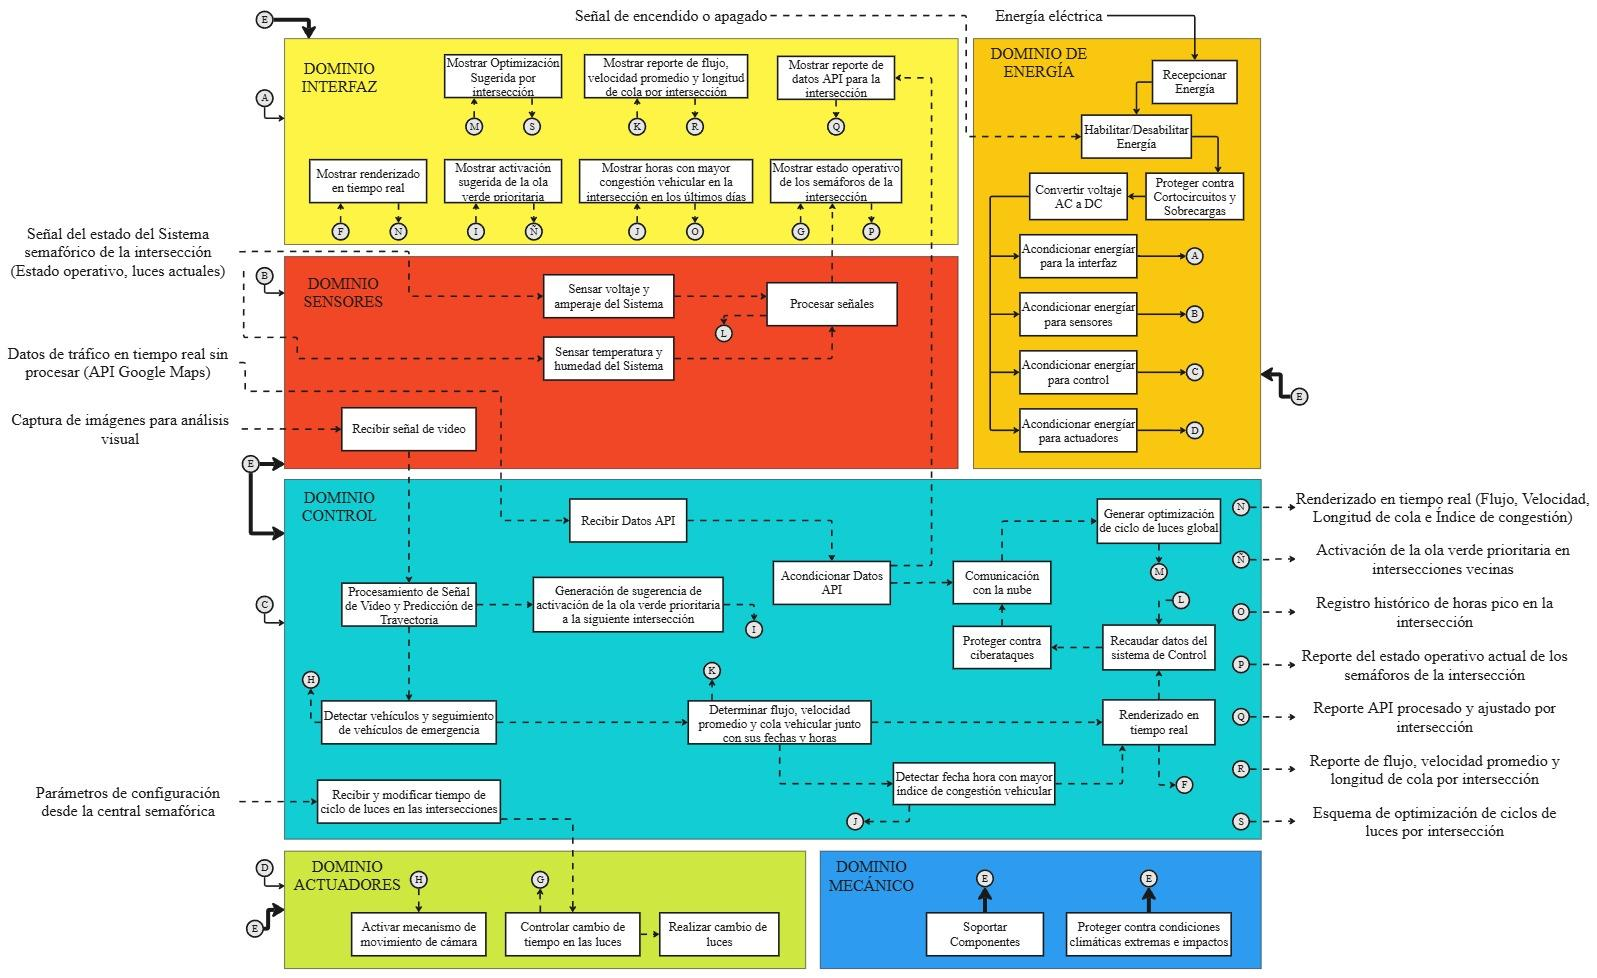
\includegraphics[width=0.9\linewidth,keepaspectratio]{media/image154.jpg}
  \caption{Estructura de funciones global del sistema, organizada por dominios.}
  \label{fig:estructura-funciones}
  \fuente{Elaboración propia.}
\end{figure}

Las señales internas que enlazan los dominios en el diagrama se identifican con letras. La
Tabla~\ref{tab:senales-funciones} reúne su significado, integrando en una sola referencia la nomenclatura que
en versiones anteriores aparecía dispersa en el texto.

\begin{table}[H]
  \centering
  \footnotesize
  \caption{Significado de las señales internas de la estructura de funciones.}
  \label{tab:senales-funciones}
  \begin{tabularx}{\linewidth}{@{}cX@{}}
    \toprule
    \textbf{Señal} & \textbf{Significado}\\
    \midrule
    A--D & Acondicionar energía para interfaz (A), sensores (B), control (C) y actuadores (D).\\
    E & Señal mecánica de soporte y protección contra condiciones extremas e impactos.\\
    F & Renderizado en tiempo real de las variables de tráfico.\\
    G & Cambio de tiempo en las luces.\\
    H & Seguimiento visual continuo del vehículo de emergencia.\\
    I & Generación de sugerencia para la activación de la ola verde prioritaria.\\
    J & Índice de congestión vehicular por fecha y hora.\\
    K & Reporte de flujo, velocidad promedio y longitud de cola por intersección.\\
    L & Datos acondicionados del estado del sistema semafórico.\\
    M & Generación de optimización del ciclo de luces global.\\
    N--S & Señales hacia la interfaz para mostrar: renderizado en tiempo real (N), activación sugerida de la ola verde (Ñ), horas de mayor congestión (O), estado operativo de los semáforos (P), reporte de datos de la API por intersección (Q), reporte de flujo, velocidad y cola (R) y optimización sugerida por intersección (S).\\
    \bottomrule
  \end{tabularx}
  \fuente{Elaboración propia.}
\end{table}

A partir de esta estructura global, cada dominio se detalla en su propio diagrama de funciones. El
\textbf{dominio de interfaz} (Figura~\ref{fig:dominio-interfaz}) agrupa las funciones de visualización para el
operador: renderizado en tiempo real, optimización sugerida por intersección, estado operativo de los
semáforos, reporte de flujo/velocidad/cola, activación sugerida de ola verde prioritaria, horas de mayor
congestión y reporte de datos de la API.

\begin{figure}[H]
  \centering
  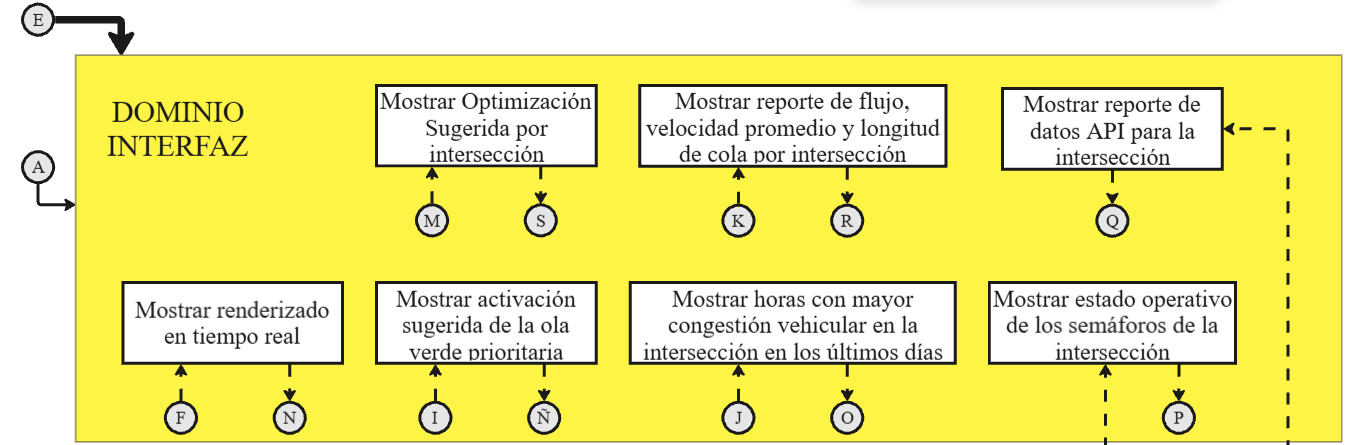
\includegraphics[width=0.9\linewidth,keepaspectratio]{media/image27.png}
  \caption{Estructura de funciones del dominio de interfaz.}
  \label{fig:dominio-interfaz}
  \fuente{Elaboración propia.}
\end{figure}
\newpage
El \textbf{dominio de sensores} (Figura~\ref{fig:dominio-sensores}) recibe la señal de video, sensa voltaje y
amperaje, sensa temperatura y humedad, y procesa las señales para detectar fallas, desconexiones o anomalías
del sistema.

\begin{figure}[H]
  \centering
  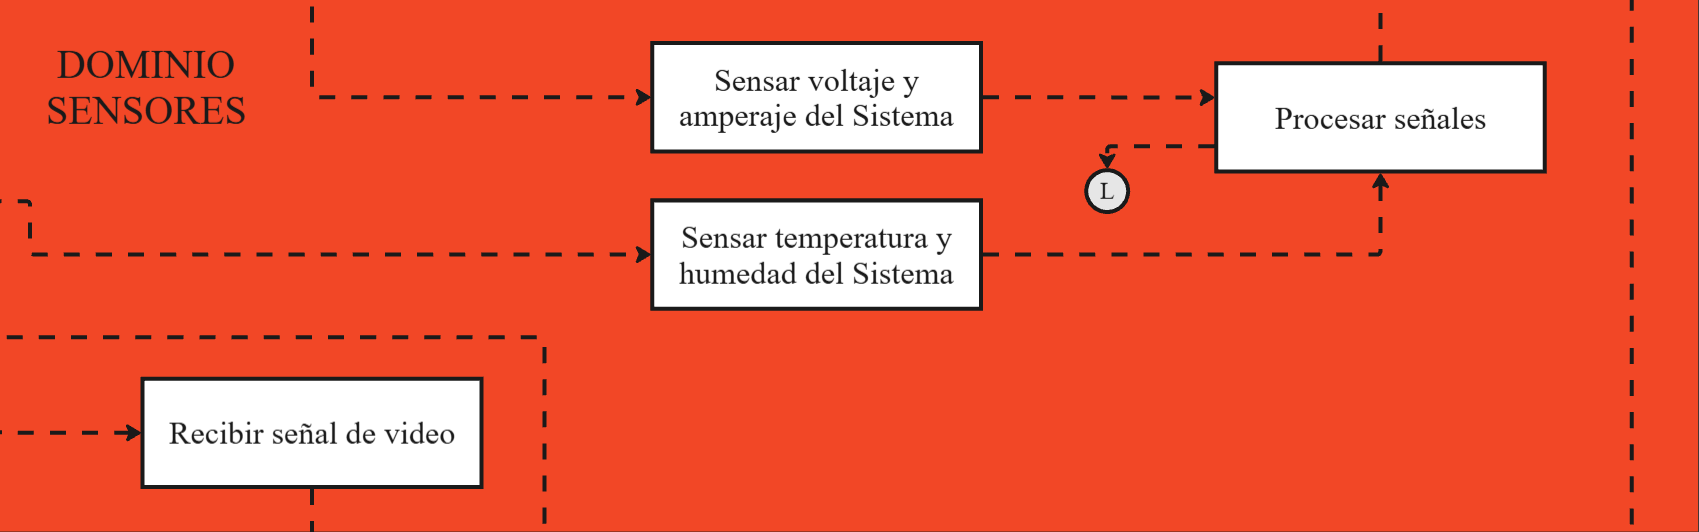
\includegraphics[width=0.9\linewidth,keepaspectratio]{media/image74.png}
  \caption{Estructura de funciones del dominio de sensores.}
  \label{fig:dominio-sensores}
  \fuente{Elaboración propia.}
\end{figure}

El \textbf{dominio de energía} (Figura~\ref{fig:dominio-energia}) recepciona la energía de la red, habilita o
deshabilita el suministro, protege contra cortocircuitos y sobrecargas, convierte AC a DC y transforma la
energía para interfaz, sensores, control y actuadores.

\begin{figure}[H]
  \centering
  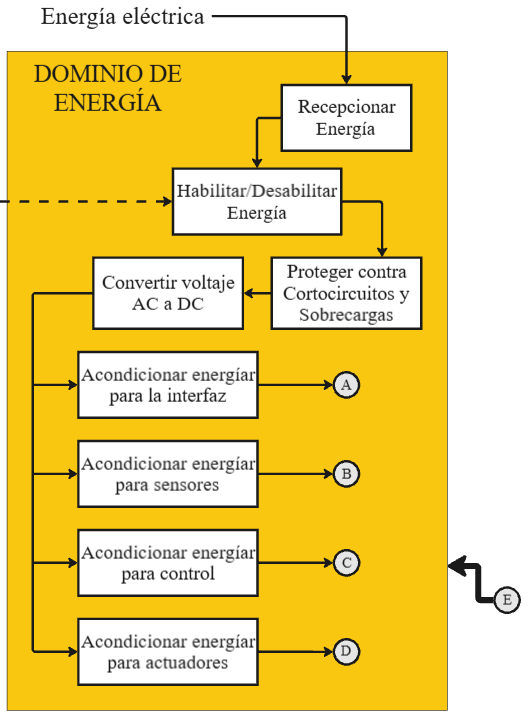
\includegraphics[width=0.4\linewidth,keepaspectratio]{media/image83.png}
  \caption{Estructura de funciones del dominio de energía.}
  \label{fig:dominio-energia}
  \fuente{Elaboración propia.}
\end{figure}

El \textbf{dominio de control} (Figura~\ref{fig:dominio-control}) constituye el núcleo: acondiciona los datos
externos, detecta y sigue vehículos, procesa el video y predice trayectorias, determina flujo, velocidad y
cola con fecha y hora, calcula el índice de congestión, genera el renderizado y las recomendaciones de
optimización, protege contra ciberataques y comunica con la nube. Sus salidas son recomendaciones acotadas,
nunca acciones directas sobre las lámparas.

\begin{figure}[H]
  \centering
  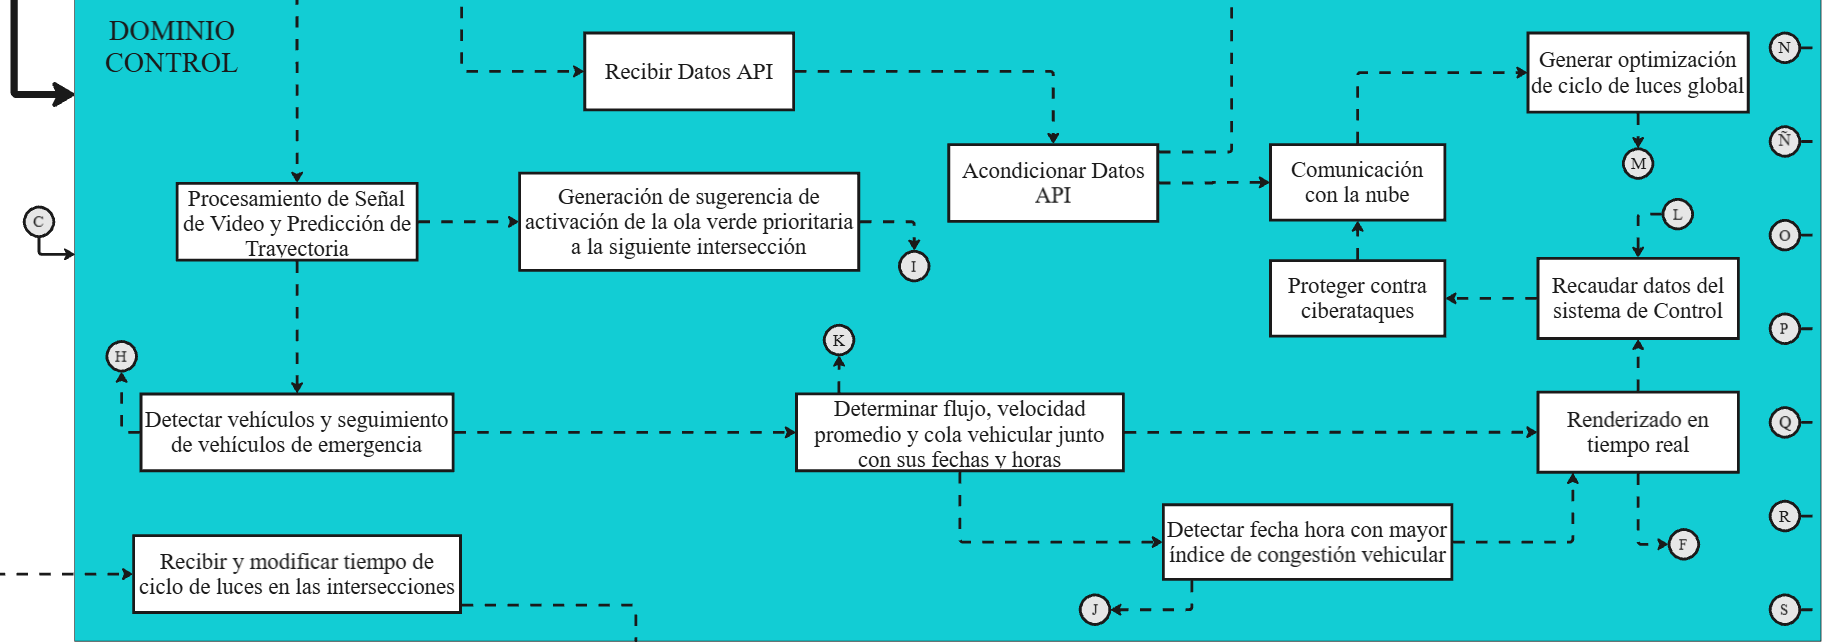
\includegraphics[width=0.9\linewidth,keepaspectratio]{media/image80.png}
  \caption{Estructura de funciones del dominio de control.}
  \label{fig:dominio-control}
  \fuente{Elaboración propia.}
\end{figure}

Finalmente, el \textbf{dominio de actuadores y el dominio mecánico} (Figura~\ref{fig:dominio-actuadores})
ejecutan, sujetos al controlador vial, el cambio de tiempos y de luces y el movimiento de la cámara, y
proveen la estructura física que soporta y protege los componentes frente a clima extremo, impactos y
vandalismo.

\begin{figure}[H]
  \centering
  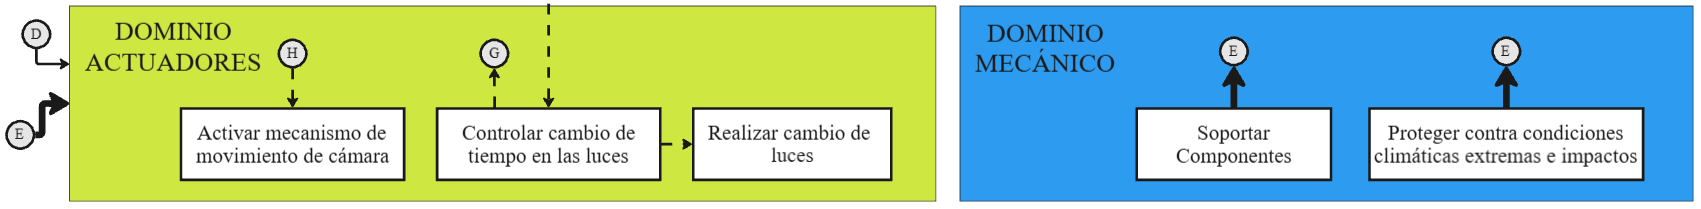
\includegraphics[width=0.9\linewidth,keepaspectratio]{media/image147.png}
  \caption{Estructura de funciones de los dominios de actuadores y mecánico.}
  \label{fig:dominio-actuadores}
  \fuente{Elaboración propia.}
\end{figure}

\section{Matriz morfológica y selección de alternativa}\label{sec:matriz-morfologica}

La matriz morfológica vincula cada función principal con tecnologías capaces de realizarla, generando cuatro
conceptos completos y comparables: \textbf{A} (control centralizado en nube), \textbf{B} (solución industrial
local cerrada), \textbf{C} (módulo complementario edge--nube) y \textbf{D} (control directo basado en
aprendizaje). Los conceptos se evaluaron técnico-económicamente en una escala de 1 a 5 ponderada por criterios
de diseño (adecuación funcional, operación local, seguridad funcional, integración, mantenibilidad,
ciberseguridad, escalabilidad, costo y facilidad de validación académica). El concepto C obtuvo la mayor
puntuación normalizada (96.4/100) por combinar autonomía local, interpretabilidad, compatibilidad con la
validación en SUMO, supervisión remota y separación de responsabilidades. La matriz morfológica completa, la
descripción de los cuatro conceptos y la evaluación ponderada detallada se presentan en el Anexo~C
(Tablas~\ref{tab:matriz-morfologica} y~\ref{tab:evaluacion-conceptos}).

Por tanto, la solución seleccionada es: \textbf{cámara con visión por computadora + procesamiento local en el
borde + índice de congestión + control difuso + comunicación segura con nube + SUMO como simulador + gabinete
modular + arquitectura complementaria al controlador existente}. Esta elección no implica que cada componente
comercial esté ya certificado; indica que el concepto satisface mejor los requerimientos del alcance de tesis.

\section{Solución óptima}\label{sec:solucion-optima}

La solución óptima corresponde al concepto C. Se trata de un módulo mecatrónico instalado en la intersección,
con cámara y gabinete de protección. La altura de instalación (del orden de 4,8\,m, según el poste dimensionado
en el Capítulo~5) y el grado IP65 se adoptan como objetivos de diseño y se confirman en la etapa de integración
mecánica (Capítulo~5). La Figura~\ref{fig:bosquejo} muestra una
visualización del concepto.

El núcleo del sistema es un módulo IoT basado en \textbf{Raspberry Pi 5}, empleado como unidad de
procesamiento local (\emph{edge}) para adquisición de datos, visión por computadora, diagnóstico y generación
de recomendaciones de control. El módulo no reemplaza al controlador semafórico existente ni asume la
autoridad final sobre los cambios de fase: lo complementa con información procesada, parámetros sugeridos y
alertas verificables por la central semafórica. Incorpora una pantalla TFT integrada que facilita el
diagnóstico del operario en sitio, mostrando únicamente el estado operativo de los semáforos y del controlador
para mantenimiento básico. El monitoreo de corriente se apoya en el sensor de efecto Hall
\textbf{WCS1600}, que mide corriente DC y AC sin contacto directo con el conductor (hasta $\pm 100$\,A DC y
70\,A RMS) y aporta aislamiento galvánico para proteger a la unidad de control; como la Raspberry~Pi~5 carece
de ADC integrado, su salida analógica se digitaliza con el \textbf{ADC MCP3008} de 10\,bits por bus SPI, lo
que habilita un mantenimiento preventivo del consumo del módulo.

El monitoreo térmico se realiza con el sensor digital de temperatura \textbf{DS18B20}, que cubre un rango de
$-55$ a $+125\,^{\circ}$C con precisión de $\pm 0{,}5\,^{\circ}$C y protocolo OneWire; su carácter digital le
confiere inmunidad al ruido electromagnético de relés y contactores y permite vigilar el sobrecalentamiento
interno del gabinete en las condiciones de Lima Metropolitana. La humedad no se mide de forma directa: el
sellado del gabinete con grado IP65 limita su ingreso por diseño.

La captura de imágenes se realiza mediante una \textbf{cámara domo fija tipo Hikvision (formato HD-TVI)} con
visión por computadora, apta para exteriores y \textbf{orientable mediante un mecanismo mecatrónico externo}
(motor paso a paso NEMA~23) que dirige su campo visual hacia los accesos Norte--Sur o Este--Oeste según la
relevancia operacional del ciclo. La cámara no incorpora un cabezal PTZ comercial integrado: su orientación es
una \emph{variable controlada} del módulo, materializada por el sistema de movimiento que se detalla en el
Capítulo~\ref{cap:diseno-mecanico}. La señal HD-TVI se digitaliza con un convertidor a USB
(Capítulo~\ref{cap:diseno-electronico}) y alimenta los algoritmos de visión que estiman flujo vehicular,
velocidad promedio y longitud de cola. La orientación preferente hacia un vehículo de emergencia se contempla
como \textbf{capacidad habilitada por la arquitectura}, no como una función validada experimentalmente en el
presente alcance. La altura de instalación y el grado IP65 se adoptan como objetivos de diseño y se confirman
en la etapa de integración mecánica (Capítulo~\ref{cap:diseno-mecanico}), donde el poste se dimensiona a
4,8\,m; la cobertura final se verifica mediante calibración geométrica de la cámara, pruebas de campo
controladas y ajuste de las zonas de detección, en especial en intersecciones con geometrías irregulares. Esta
cámara domo orientable es la \textbf{única solución de visión} empleada de forma consistente en todo el
documento.

\begin{figure}[H]
  \centering
  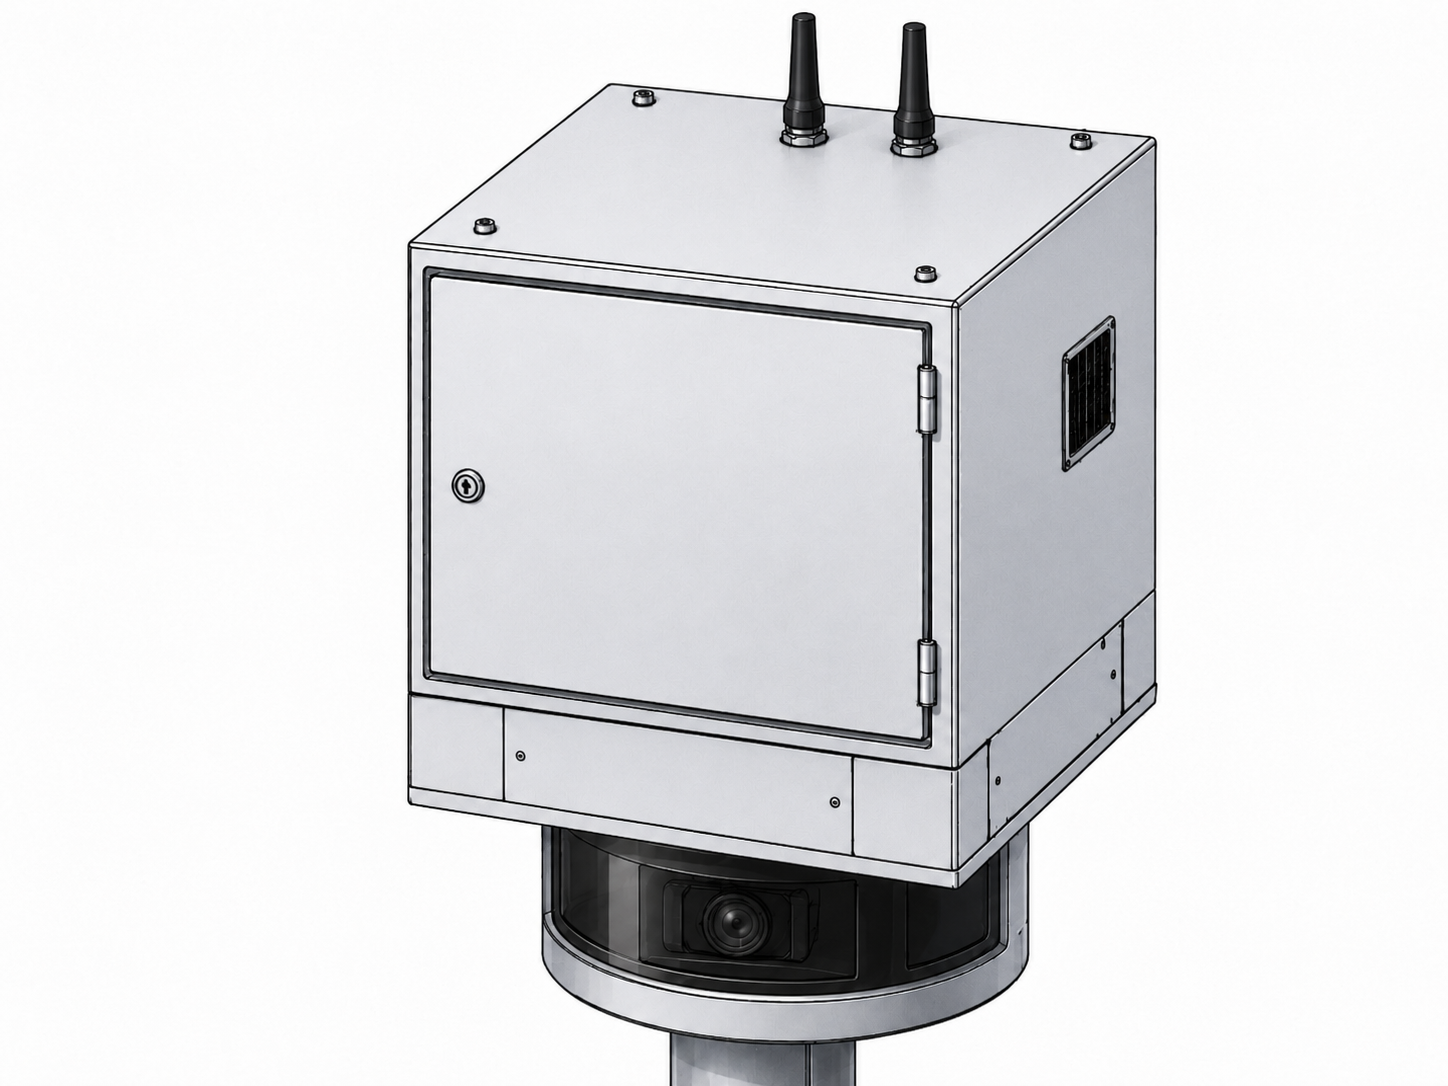
\includegraphics[width=0.4\linewidth,keepaspectratio]{media/image140.png}
  \caption{Bosquejo del diseño de la solución óptima.}
  \label{fig:bosquejo}
  \fuente{Elaboración propia.}
\end{figure}

Para el banco de pruebas y la etapa de diseño electrónico se considera una interfaz de conmutación mediante
relés de estado sólido (SSR), por su conmutación silenciosa y ausencia de desgaste mecánico. En una
implementación vial real, la actuación final de las luces permanece condicionada por el controlador
semafórico certificado, sus enclavamientos de seguridad y las restricciones normativas aplicables. La
iluminación semafórica se plantea mediante un sistema de fibra óptica LED que distribuye uniformemente la luz
desde la base del controlador hacia los focos, lo que facilita el mantenimiento.

La alimentación del sistema incorpora llaves termomagnéticas, protección diferencial o equivalente según la
instalación, una fuente AC/DC y convertidores DC/DC para los niveles requeridos. El respaldo mediante batería
o UPS se dimensiona con el perfil de carga en el Capítulo~4. La comunicación entre el controlador programable
y la central semafórica, y entre el controlador y el módulo IoT, se establece mediante el protocolo
\textbf{NTCIP} sobre TCP/IP; la comunicación entre el módulo IoT y la nube usa el protocolo \textbf{MQTT} sobre
TCP/IP con TLS, priorizando una transmisión eficiente y segura sin requerir comunicación bidireccional
constante.

El procesamiento local se plantea con OpenCV y un detector de objetos ejecutado en la unidad \emph{edge}, para
estimar flujo, velocidad y cola. La detección de vehículos de emergencia es una función complementaria cuya
precisión se valida con un conjunto de datos específico. \textbf{Microsoft Azure} se emplea como plataforma de
referencia para almacenamiento, supervisión y recomendaciones de coordinación, sin eliminar la validación
local ni la autoridad final del controlador. La arquitectura de ciberseguridad considera cifrado en tránsito,
gestión de identidades y accesos, MFA para operadores, registro de eventos y separación de redes o zonas de
confianza; su efectividad se verifica en un banco de integración y mediante pruebas autorizadas, sin que el
presente diseño acredite una certificación.

\subsection{Justificación de la cámara orientable como estrategia de percepción activa}
\label{subsec:percepcion-activa}

La selección de una cámara orientable no responde únicamente a la sustitución de una configuración con
múltiples cámaras fijas, sino a la adopción de una estrategia de \emph{percepción activa}. En una intersección
semaforizada, la información visual requerida por el sistema no tiene la misma relevancia durante todo el ciclo
de operación: durante el rojo resulta prioritario observar la formación de colas; durante el verde, la descarga
vehicular; y, en condiciones de saturación, el eje con mayor demanda acumulada. Por ello, la orientación de la
cámara se incorpora como una variable controlada del módulo mecatrónico, lo que permite dirigir el campo visual
hacia el eje de mayor relevancia operacional.

Mientras una configuración de cámaras fijas vigila de forma permanente zonas predefinidas, la cámara orientable
actualiza de manera selectiva los accesos Norte--Sur y Este--Oeste en función del estado de la intersección,
del nivel de congestión estimado o de una condición prioritaria. Esta decisión es coherente con el
carácter complementario del módulo, ya que el sistema no acciona directamente las luces, sino que estima
variables de tráfico y genera recomendaciones acotadas para el controlador semafórico existente. Asimismo, la
movilidad de la cámara permite trabajar con regiones de interés más específicas y con mejor resolución efectiva
sobre el eje observado, en lugar de depender de una vista excesivamente amplia donde los vehículos pueden
aparecer pequeños, parcialmente ocluidos o afectados por una perspectiva desfavorable. Al emplear un único
sensor físico se mantiene además una cadena de visión homogénea: misma óptica, mismo detector y parámetros de
calibración definidos por orientación, lo que evita discrepancias entre sensores distintos.

En escenarios prioritarios, la arquitectura también habilita políticas de orientación preferente. Por ejemplo,
si el sistema recibe una señal externa o una futura detección confiable asociada a un vehículo de emergencia, la
cámara puede orientarse hacia el acceso correspondiente para verificar cola, trayectoria y condiciones de
despeje. Esta capacidad se plantea como una extensión funcional habilitada por la arquitectura, no como una
validación experimental dentro del presente alcance. Desde el punto de vista mecatrónico, la cámara orientable
integra percepción, electrónica de control, mecanismo de posicionamiento, selección de actuador, rigidez
estructural y lógica de decisión local; por tanto, no constituye un accesorio, sino un elemento que vincula los
dominios mecánico, electrónico y de control del módulo propuesto. La Tabla~\ref{tab:camara-orientable} resume
esta comparación funcional, sin recurrir a argumentos de costo o de cableado.

\begin{table}[H]
  \centering
  \footnotesize
  \caption{Comparación funcional entre una configuración de cámaras fijas y una cámara orientable.}
  \label{tab:camara-orientable}
  \begin{tabularx}{\linewidth}{@{}>{\raggedright\arraybackslash}p{3.0cm}XX@{}}
    \toprule
    \textbf{Criterio} & \textbf{Dos cámaras fijas} & \textbf{Una cámara orientable}\\
    \midrule
    Tipo de percepción & Observación pasiva y simultánea de regiones predefinidas. & Percepción activa dirigida hacia el eje operacionalmente relevante.\\
    Relación con el ciclo semafórico & Captura permanente, independiente de la fase. & Sincroniza la observación con la formación de cola, la descarga vehicular o la saturación.\\
    Calidad visual por eje & Depende de una vista amplia o de condiciones de instalación distintas entre cámaras. & Enfoca regiones de interés específicas con una cadena de visión homogénea.\\
    Consistencia de calibración & Requiere mantener la consistencia entre sensores. & Emplea el mismo sensor y una calibración definida por orientación.\\
    Eventos prioritarios & Selecciona entre flujos de video ya existentes. & Orienta activamente el campo visual hacia el acceso prioritario.\\
    Aporte mecatrónico & Predomina el sensado fijo y el procesamiento de video. & Integra sensado, control de orientación, mecanismo, actuador y decisión local.\\
    \bottomrule
  \end{tabularx}
  \fuente{Elaboración propia.}
\end{table}

En consecuencia, la elección de una cámara orientable no se plantea como una solución universalmente superior a
una arquitectura multicámara, sino como una decisión de diseño alineada con el objetivo de esta tesis: proponer
un módulo IoT mecatrónico complementario, capaz de sensar activamente la intersección, actualizar variables
locales y entregar recomendaciones acotadas sin sustituir la autoridad del controlador semafórico existente.

\subsection{Arquitectura general y flujo del sistema}\label{sec:arquitectura-flujo}

La Figura~\ref{fig:flujo-general} resume el flujo general. El controlador vial acciona las salidas de campo
mediante sus interfaces eléctricas y conserva los enclavamientos. NTCIP sobre TCP/IP se utiliza para el
intercambio de estado y parámetros con la central o el módulo cuando el equipo instalado lo soporte; no es el
enlace eléctrico hacia las lámparas. El módulo IoT recopila datos locales, genera recomendaciones acotadas y
comunica telemetría con la nube mediante MQTT/TLS. La nube cumple un rol de análisis adaptativo global,
accediendo a los datos de los distintos módulos IoT distribuidos para calcular estrategias de coordinación más
eficientes, y se conecta a la central semafórica supervisora, que a su vez mantiene comunicación directa con
el controlador programable.

\begin{figure}[H]
  \centering
  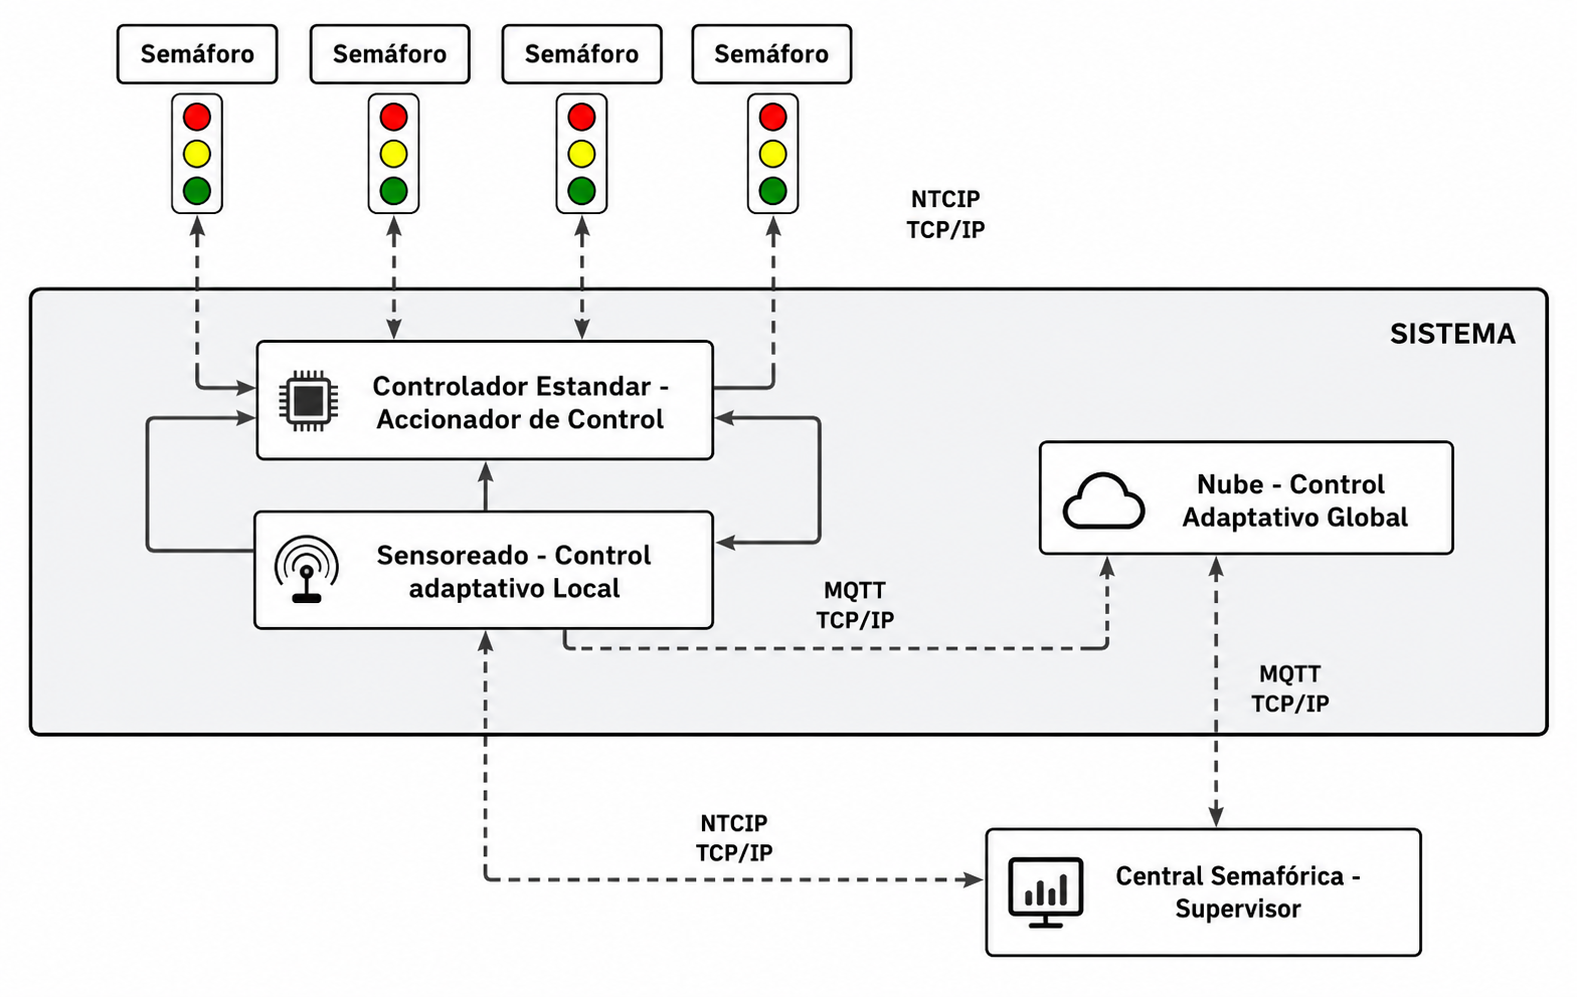
\includegraphics[width=0.7\linewidth,keepaspectratio]{media/image49.png}
  \caption{Diagrama general de flujo del sistema.}
  \label{fig:flujo-general}
  \fuente{Elaboración propia.}
\end{figure}

El módulo IoT actúa como intermediario entre el controlador programable y la nube, facilitando la recolección
y transmisión de datos del entorno local hacia el sistema de control superior. Esta intermediación permite una
comunicación fluida incluso cuando los controladores pertenecen a distintas marcas y protocolos, mitigando la
fragmentación tecnológica existente en Lima, donde coexisten diferentes fabricantes (SICE, SUTEC, ORIUX,
SWARCO) y múltiples protocolos (AENOR, OPCT, NTCIP, BEFA). No obstante, en esta tesis no se implementa ni
certifica la integración con un controlador comercial específico: la compatibilidad NTCIP se plantea como
arquitectura de interfaz y la salida del módulo permanece como recomendación acotada; la interfaz física y
protocolar con un controlador real debe verificarse en un banco \textit{hardware-in-the-loop} y en un piloto
controlado. Las Figuras~\ref{fig:flujo-completo} y~\ref{fig:flujo-completo-b} detallan la
lógica operativa completa: el sistema inicia con la energización y verificación de la fuente, la inicialización
secuencial del controlador interno, la activación de la cámara, los sensores de monitoreo ambiental y
energético y los actuadores; tras verificar la comunicación, entra en un bucle continuo que captura imágenes,
detecta flujo, velocidad y cola, calcula el índice de congestión, ejecuta la rutina de detección de vehículos
de emergencia y, en su caso, genera la sugerencia de ola verde prioritaria, acondicionando y cifrando los
datos para su transmisión segura a la nube.

\begin{figure}[H]
  \centering
  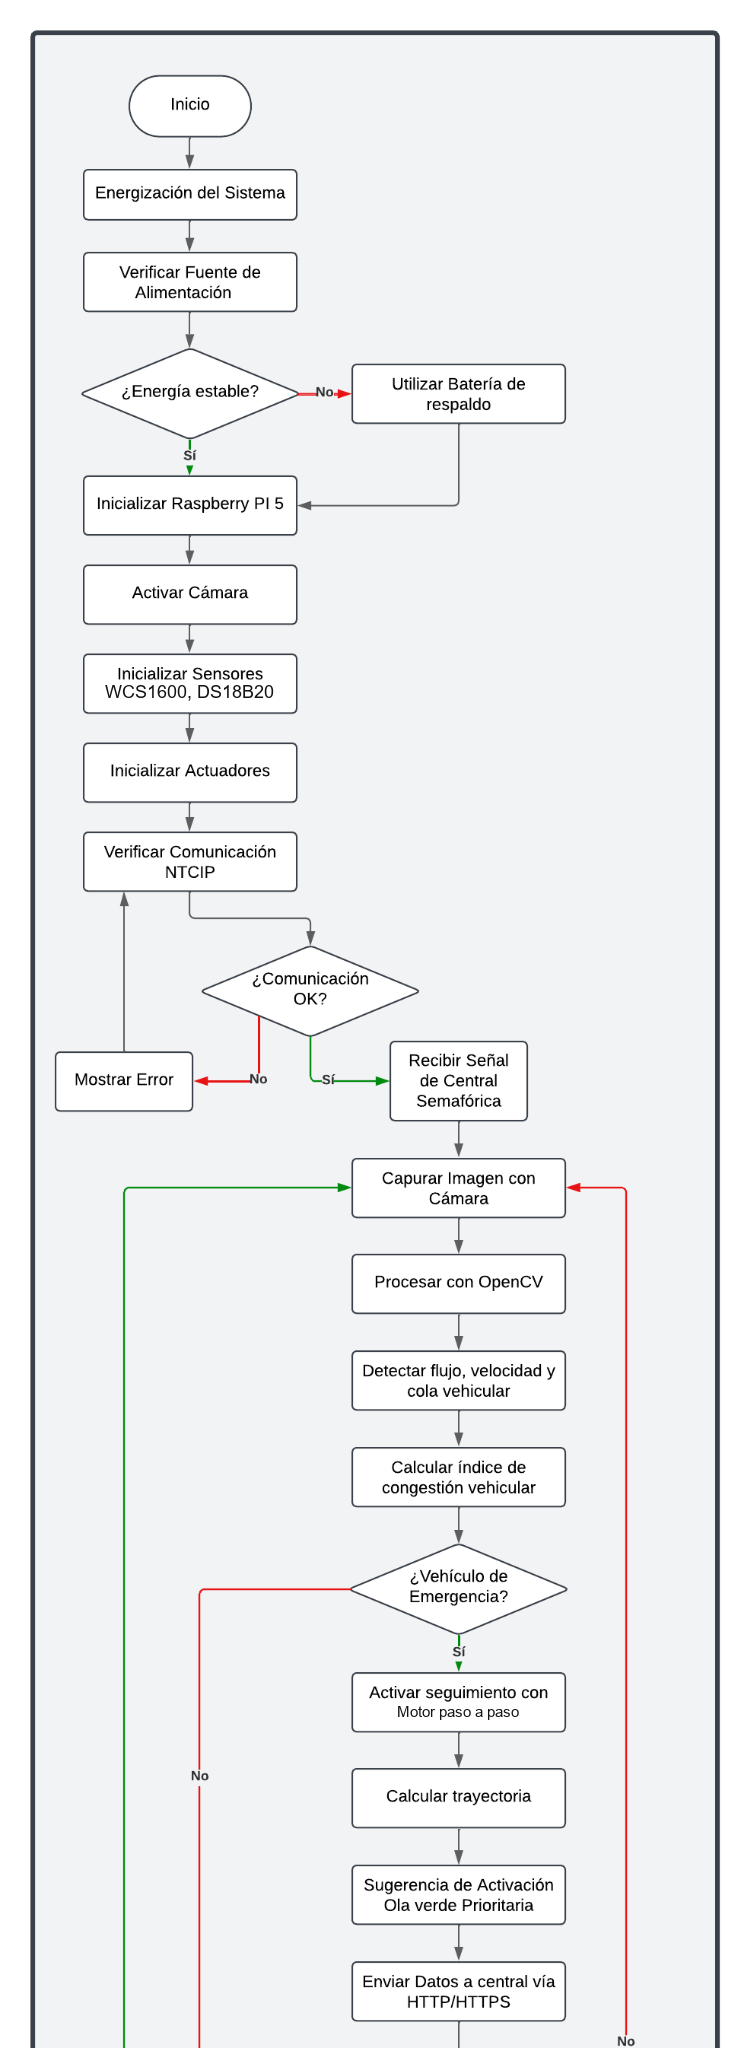
\includegraphics[width=0.4\linewidth,keepaspectratio]{media/image66.png}
  \caption{Diagrama del flujo completo del sistema (parte~1 de~2): energización,
  inicialización de subsistemas y verificación de la comunicación.}
  \label{fig:flujo-completo}
  \fuente{Elaboración propia.}
\end{figure}

\begin{figure}[H]
  \centering
  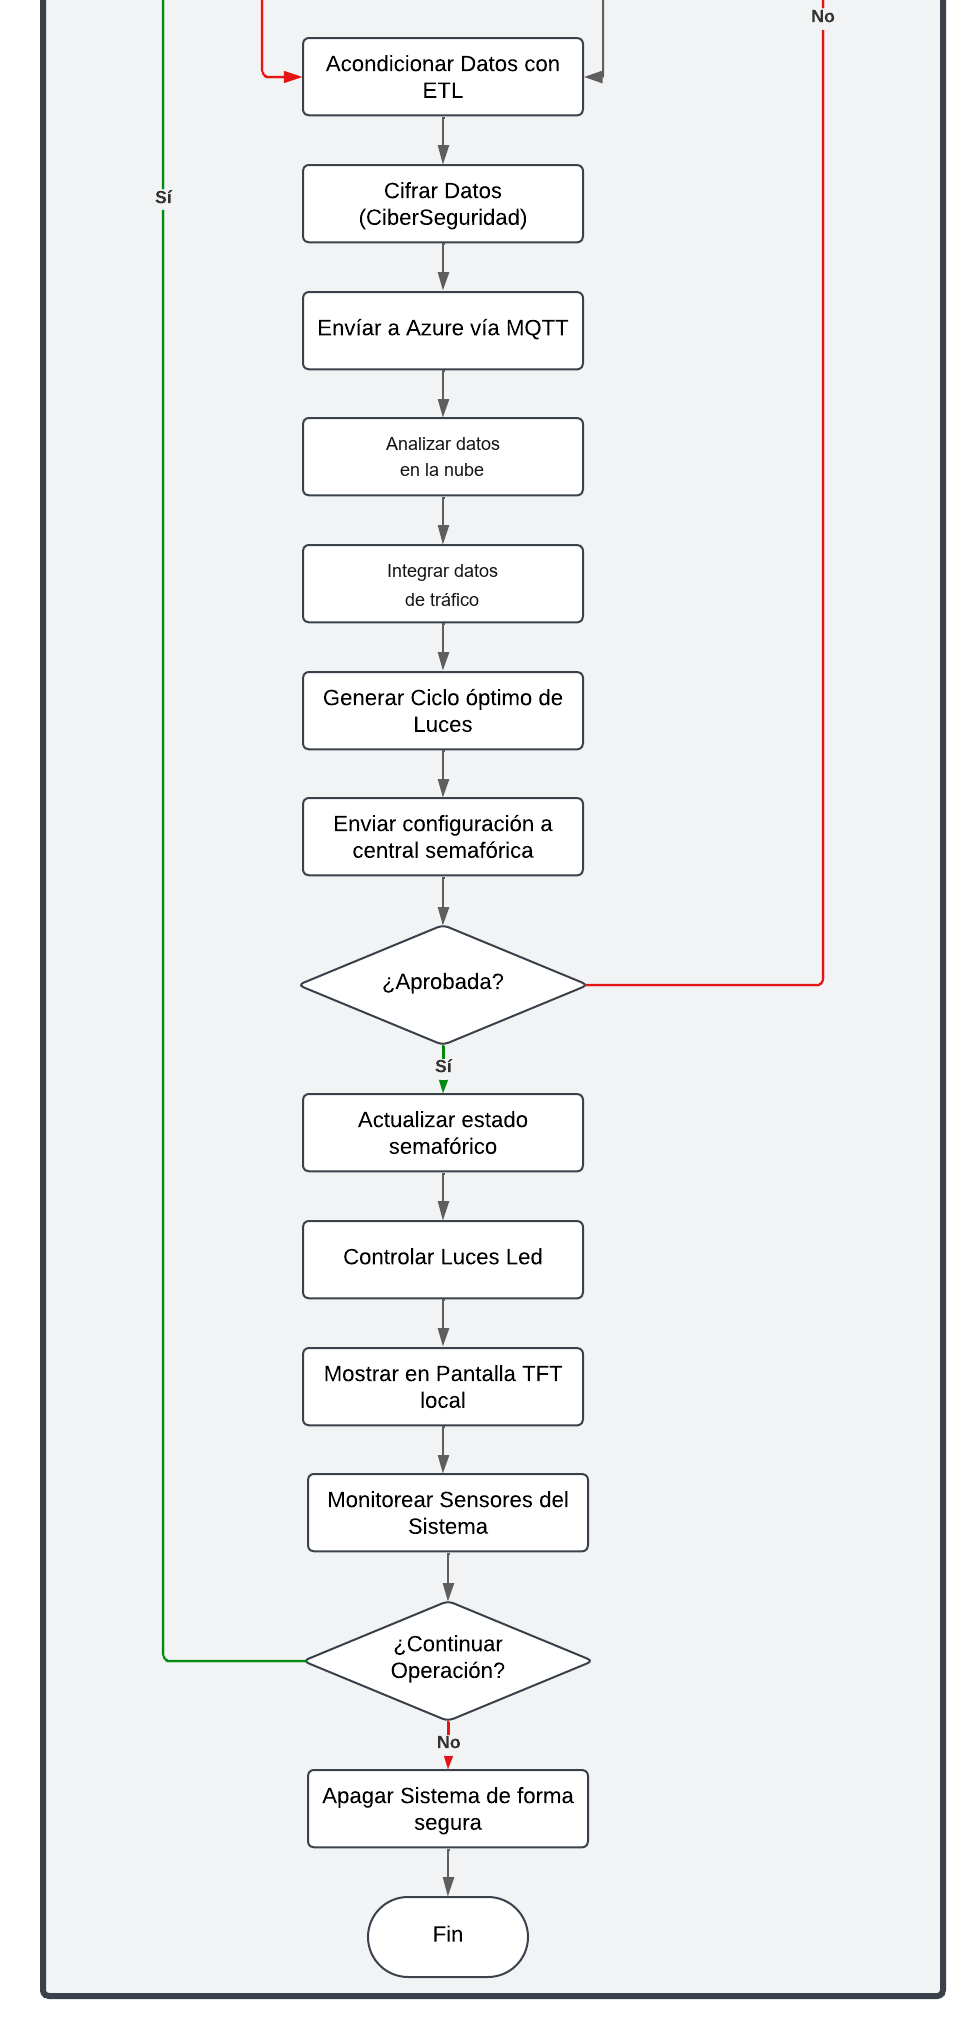
\includegraphics[width=0.4\linewidth,keepaspectratio]{media/image33.png}
  \caption{Diagrama del flujo completo del sistema (parte~2 de~2): bucle de captura,
  cálculo del índice de congestión y transmisión segura hacia la nube.}
  \label{fig:flujo-completo-b}
  \fuente{Elaboración propia.}
\end{figure}

El diagrama de bloques de la solución (Figura~\ref{fig:diagrama-bloques}) evidencia la arquitectura integral
distribuida entre procesamiento local y nube; su leyenda, que separa líneas de alimentación y de señal y
diferencia por colores cada dominio, se presenta en la Figura~\ref{fig:leyenda-bloques}. El sistema se
estructura en torno a la unidad de procesamiento local Raspberry Pi 5, complementada con aceleración o
periféricos de procesamiento de imágenes cuando el desempeño de visión lo requiera, y se conecta con la nube
Azure para análisis, almacenamiento y recomendaciones de coordinación. La alimentación parte de la red de
220\,V AC, protegida por llaves termomagnéticas y disyuntores, convertida mediante una fuente conmutada AC/DC
de 24\,V, complementada con batería DC de respaldo y convertidores DC/DC. El monitoreo ambiental y energético
emplea los sensores WCS1600 (con ADC MCP3008) y DS18B20, y la captura visual la cámara domo fija orientable por mecanismo externo; la
comunicación opera con NTCIP hacia la central de control y MQTT hacia la nube Azure.

\begin{figure}[H]
  \centering
  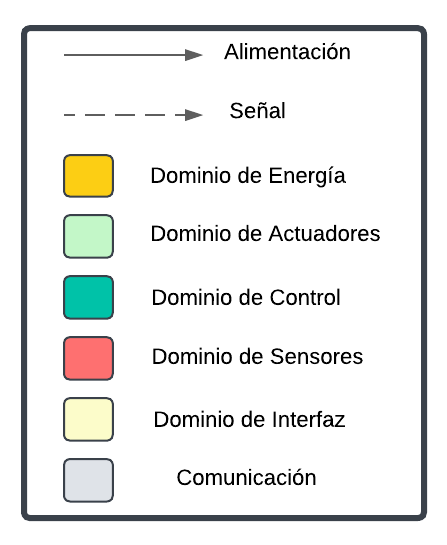
\includegraphics[width=0.3\linewidth,keepaspectratio]{media/image13.png}
  \caption{Leyenda del diagrama de bloques del sistema.}
  \label{fig:leyenda-bloques}
  \fuente{Elaboración propia.}
\end{figure}

\begin{figure}[H]
  \centering
  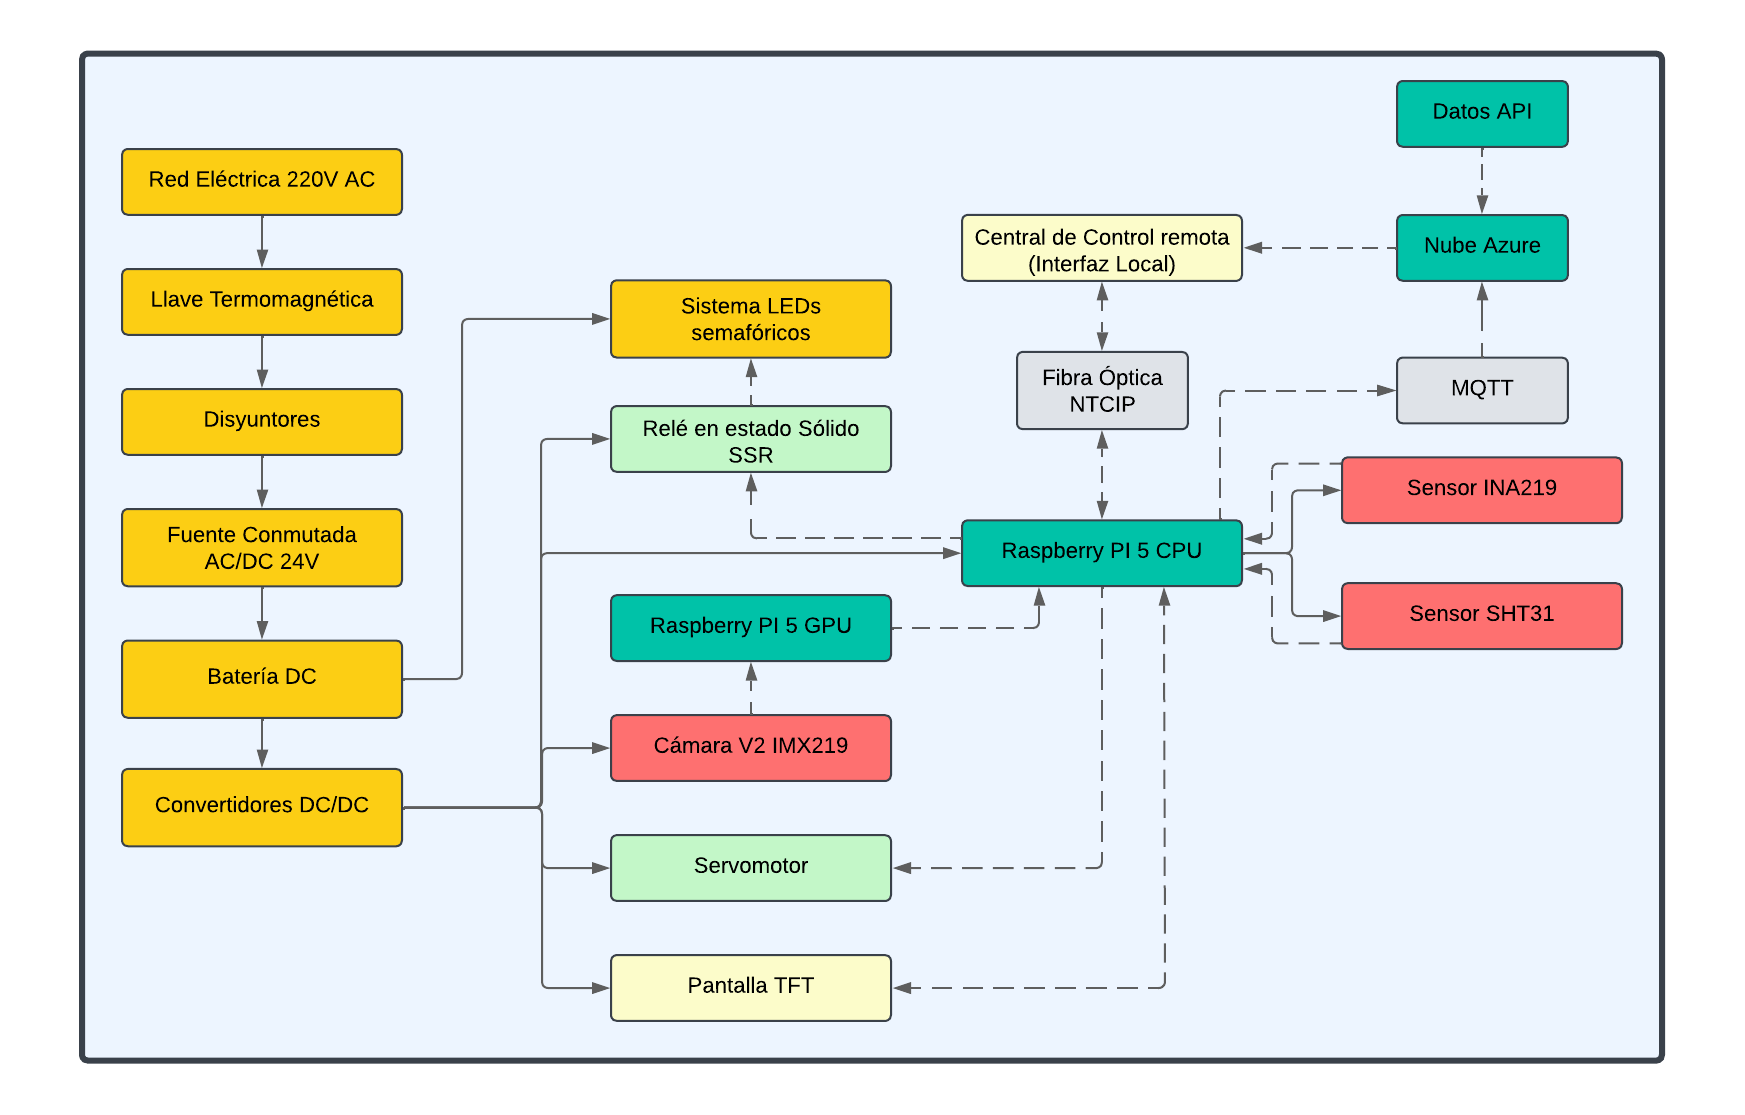
\includegraphics[width=0.9\linewidth,keepaspectratio]{media/image151.png}
  \caption{Diagrama de bloques del sistema.}
  \label{fig:diagrama-bloques}
  \fuente{Elaboración propia.}
\end{figure}

\subsection{Jerarquía de alcance y responsabilidad}\label{sec:jerarquia-alcance}

La solución se organiza en niveles de alcance que separan el núcleo validado de los módulos exploratorios. La
relación \emph{edge}--nube--controlador es jerárquica: la cámara y los sensores alimentan la estimación y el
control difuso en el borde; el borde envía telemetría segura a la nube (supervisión, históricos y coordinación)
y recomendaciones acotadas al controlador semafórico, que conserva la autoridad final sobre luces y
enclavamientos; la nube y la central devuelven únicamente parámetros autorizados. La
Tabla~\ref{tab:niveles-alcance} detalla los niveles y la evidencia esperada de cada uno.

\begin{table}[H]
  \centering
  \footnotesize
  \caption{Niveles de alcance del sistema y evidencia esperada.}
  \label{tab:niveles-alcance}
  \begin{tabularx}{\linewidth}{@{}>{\raggedright\arraybackslash}p{3.5cm}>{\raggedright\arraybackslash}X>{\raggedright\arraybackslash}p{4.6cm}@{}}
    \toprule
    \textbf{Nivel} & \textbf{Contenido} & \textbf{Evidencia esperada}\\
    \midrule
    Nivel 1: núcleo validado & Sensado/variables equivalentes, ICV, control difuso local, diseño electrónico y mecánico, SUMO y comparación con línea base. & Ecuaciones, reglas, esquemas, CAD, simulaciones y tabla comparativa.\\
    Nivel 2: arquitectura de soporte & Comunicación con nube, supervisión, histórico, alertas y actualización autorizada de parámetros. & Arquitectura, mensajes, dashboard y prueba controlada.\\
    Nivel 3: seguridad y operación & Modelo de amenazas, cifrado, autenticación, roles, logs, validación de parámetros y modos degradados. & Tabla de amenazas, flujo de confianza y casos negativos.\\
    Nivel 4: módulos exploratorios/futuros & Aprendizaje por refuerzo, CNN--LSTM, optimización metropolitana, reentrenamiento continuo e integración comercial certificada. & Propuesta o experimento separado; no condiciona el objetivo general.\\
    \bottomrule
  \end{tabularx}
  \fuente{Elaboración propia.}
\end{table}

\subsection{Riesgos y limitaciones del concepto edge--nube}\label{sec:riesgos-concepto}

La arquitectura seleccionada presenta riesgos y limitaciones que condicionan su implementación y se gestionan
con las mitigaciones de la Tabla~\ref{tab:riesgos-concepto}. Estas mitigaciones se trazan con los
requerimientos verificables (Tabla~\ref{tab:req-verificables}) y se ejercitan durante la validación.

\begin{table}[H]
  \centering
  \footnotesize
  \caption{Riesgos y limitaciones del concepto edge--nube y sus mitigaciones.}
  \label{tab:riesgos-concepto}
  \begin{tabularx}{\linewidth}{@{}>{\raggedright\arraybackslash}p{3.6cm}>{\raggedright\arraybackslash}X>{\raggedright\arraybackslash}p{2.0cm}@{}}
    \toprule
    \textbf{Riesgo o limitación} & \textbf{Mitigación de diseño} & \textbf{Requisito}\\
    \midrule
    Pérdida de conectividad con la nube & Decisión local en el borde y retorno determinista al plan base; almacenamiento local y reintento de conexión. & R-C01, R-C04, R-VAL03\\
    Falla o descalibración de sensores/cámara & Diagnóstico interno, modo degradado ante datos inválidos y pruebas periódicas de calibración. & R-C04, R-F01\\
    Oclusión o geometría irregular de la intersección & Calibración geométrica, ajuste de zonas de detección y verificación de cobertura en campo. & R-MEC03\\
    Errores del algoritmo de optimización & Recomendaciones acotadas por límites de fase; el controlador valida antes de aplicar y mantiene la autoridad final. & R-C02, R-C03\\
    Ciberataque o manipulación de parámetros & Cifrado en tránsito, identidad por dispositivo, lista blanca de parámetros, roles y registro de eventos. & R-SEC01--R-SEC04, R-COM02\\
    Transitorios eléctricos y cortes de energía & Protecciones dimensionadas y respaldo por batería/UPS para apagado controlado. & R-ELEC01, R-ELEC02\\
    Heterogeneidad de controladores en Lima & Módulo IoT como intermediario que abstrae marcas y protocolos sin sustituir la lógica local. & R-COM01, R-OP01\\
    Sobrecosto frente al presupuesto objetivo & Componentes disponibles y de bajo costo; estimación de CAPEX/OPEX y análisis de sensibilidad. & R-COST01\\
    \bottomrule
  \end{tabularx}
  \fuente{Elaboración propia.}
\end{table}

\section{Matriz de trazabilidad de objetivos}\label{sec:trazabilidad-objetivos}

Finalmente, la Tabla~\ref{tab:trazabilidad} vincula los objetivos específicos con los requerimientos, los
capítulos donde se abordan, el método de validación y la evidencia esperada, cerrando la trazabilidad entre el
diseño conceptual y las etapas de desarrollo y validación.

\begin{landscape}
\begin{table}[!htbp]
\centering
\footnotesize
\centering
\caption{Trazabilidad entre objetivos, requerimientos y evidencia.}\label{tab:trazabilidad}
\begin{tabular}{@{}p{1.3cm}p{4.3cm}p{2.6cm}p{3.7cm}p{7.0cm}@{}}
\toprule
\textbf{Objetivo} & \textbf{Requerimientos relacionados} & \textbf{Capítulos} & \textbf{Método de validación} & \textbf{Evidencia/resultado}\\
\midrule
OE1 & Base para todos los requerimientos & 1 y 2 & Revisión comparativa y síntesis & Tabla de lecciones y criterios adoptados.\\
OE2 & R-F01 a R-COST01 & 3 & Inspección de especificación & Tabla~\ref{tab:req-verificables} con código, criterio, justificación y verificación.\\
OE3 & R-C01, R-C02, R-C04, R-COM01, R-MEC01 & 3 & Evaluación ponderada & Caja negra, estructura funcional, matriz morfológica y concepto C.\\
OE4 & R-ELEC01 a R-ELEC03, R-COM01 & 4 & Cálculo y revisión de diseño & Esquemas, consumo, selección de componentes y protecciones.\\
OE5 & R-MEC01 a R-MEC03, R-CAM01 & 5 & CAD, cálculo y simulación & Distribución, soporte, sistema de orientación, análisis térmico/estructural y factor de seguridad.\\
OE6 & R-F02, R-C01, R-C03, R-C04, R-CAM02--R-CAM04 & 6 & Casos de prueba y SUMO & Membresías, reglas, superficie, saturaciones, política de orientación y modos degradados.\\
OE7 & R-COM01, R-COM02, R-NUB01 & 6 y 7 & Demostración controlada & Flujo de mensajes, histórico, alertas y prueba de desconexión.\\
OE8 & R-SEC01 a R-SEC04 & 2, 6 y 7 & Análisis de amenazas & Tabla de amenazas, mitigaciones y evidencia de controles propuestos.\\
OE9 & R-VAL01 a R-VAL03 & 7 & Simulación comparativa & Tabla comparativa de métricas SUMO y archivos de salida del Capítulo~7.\\
OE10 & R-COST01 & 7 & Presupuesto y sensibilidad & CAPEX/OPEX con fuentes, fecha y supuestos.\\
\bottomrule
\end{tabular}
\fuente{Elaboración propia.}
\end{table}
\end{landscape}
